% Dokumentum konfiguráció
\documentclass[fleqn,12pt]{article}
% --------------------------------------------------
% Dokumentum adatok
% --------------------------------------------------

% Intézmény és kar
\newcommand\INTEZMENY{Budapesti Műszaki és Gazdaságtudományi Egyetem}
\newcommand\KAR{Gépészmérnöki Kar}
\newcommand\LOGO{bme-logo.jpg} % logo fájl neve a figures mappában

% Dokumentum adatok
\newcommand\CIM{Grundlagen der Mechatronik Hausaufgabe}
\newcommand\DATUM{2025/26/1}
\newcommand\NEV{Abos Gergő}
\newcommand\NEPTUN{C46M9M}
\newcommand\EMAIL{gergo.abos@gmail.com}
\newcommand\TANTARGY{Grundlagen der Mechatronik}
\newcommand\TANTARGYKOD{BMEGEMIBSMMALP-01}

% --------------------------------------------------
% Preambulum és egyéni parancsok betöltése
% --------------------------------------------------

\input{../_settings/00_preambulum.tex}
\input{../_settings/01_commands.tex}
\input{../_settings/02_mechTikz.tex}

% ==================================================
% Dokumentum kezdete
% ==================================================
\begin{document}

% Címlap és tartalomjegyzék
% \input{contents/01_title.tex}
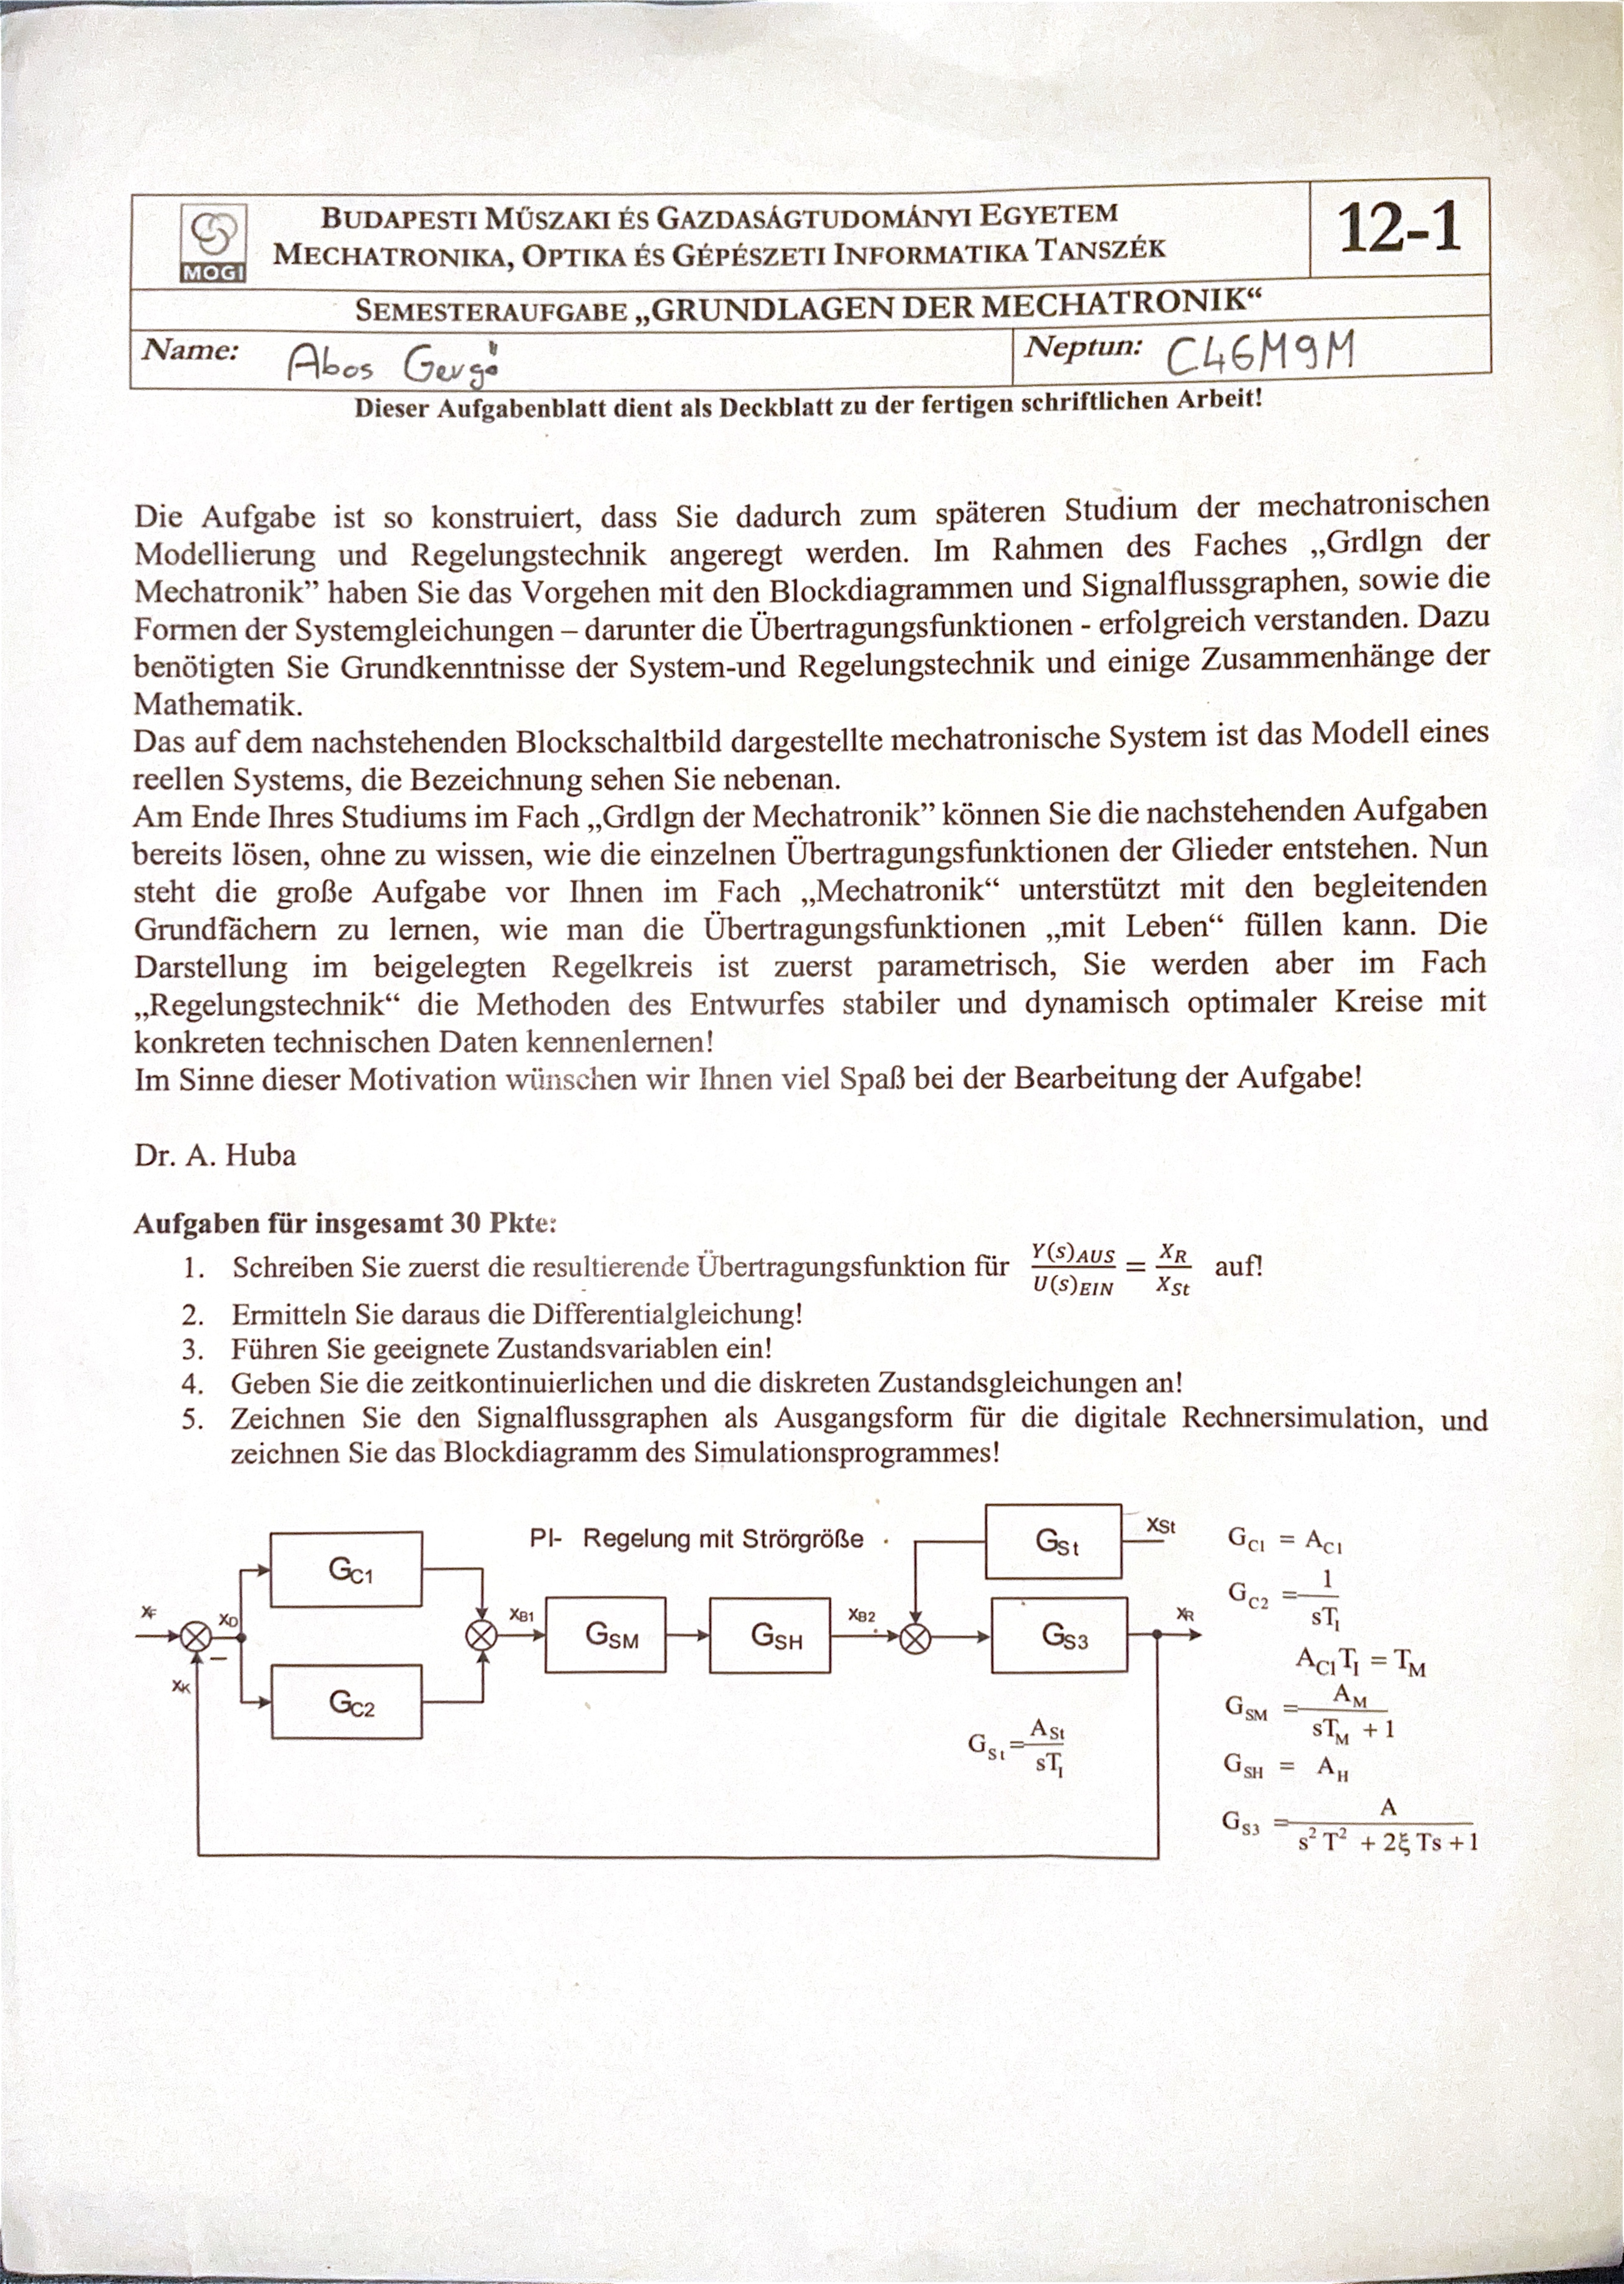
\includepdf[pages=1]{contents/Aufgabenblatt.pdf} % feladatlap beszúrása, ha szükséges
% \input{contents/02_contentpage.tex}
\section{Übertragungsfunktion}
\subsection{Parametrisch}
Wenn zwei Übertragungsglieder nacheinander schaltet sind, werden die zwei Übertragungsfunktionen multipliziert. Wenn sie parallel schaltet sind, werden die zwei Funktionen addiert.

Gesucht ist $\frac{X_R}{X_{St}}$. Deswegen wird $X_F$ als $0$ genehmen, es wird nicht in die Gleichung geschrieben werden.

\begin{align*}
  G_C &= G_{C1} + G_{C2} \\
  G_S &= G_{SM} \cdot G_{SH} \\
  G_{Vor} &= G_C \cdot G_S
\end{align*}

Damit ist das System so vereinfacht:
\begin{figure}[H]
  \centering
  \begin{tikzpicture}[
      % Define block styles
      block/.style={rectangle, thick, draw, minimum height=1cm, minimum width=2cm, align=center},
      signal/.style={thick, ->},
      >=stealth
    ]
    \coordinate (Gvor) at (6, -2);
    \coordinate (GSt) at (2, 0);
    \coordinate (GS3) at (6, 0);
    \draw[signal] (0,0) -- (1, 0) node[above left] {$X_{St}$};
    \draw[signal] (3,0) -- (3.75, 0);
    \draw[signal] (4.25,0) -- (5, 0);
    \draw[signal] (7,0) -- (9, 0) node [above left] {$X_R$};
    \draw[signal] (8,0) -- (8, -2) -- (7, -2);
    \draw[signal] (5,-2) -- (4, -2) -- (4, -0.25);
    \fill (8, 0) circle (0.1);
    \draw [thick] (4, 0) circle (0.25);
    \draw [thick] ($(4, 0) + (45:0.25)$) -- ($(4, 0) + (225:0.25)$);
    \draw [thick] ($(4, 0) + (135:0.25)$) -- ($(4, 0) + (-45:0.25)$) node[below] {-};
    \node[block] at (Gvor) {$G_{Vor}$};
    \node[block] at (GSt) {$G_{St}$};
    \node[block] at (GS3) {$G_{S3}$};
  \end{tikzpicture}
\end{figure}

Davon kann die Übertragungsfunktion mit dem Formel bestimmt werden:
\begin{align*}
  G(s) = \frac{X_R}{X_{St}} = \frac{G_{St} \cdot G_{S3}}{1 + G_{S3} \cdot G_{Vor}} =
  \frac{G_{St} \cdot G_{S3}}{1 + G_{S3} \cdot (G_{C1} + G_{C2}) \cdot G_{SM} \cdot G_{SH}}
\end{align*}
\subsection{Numerisch}
\begin{align*}
  G_C &= A_{C1} + \frac{1}{sT_I}\\
  G_S &= \frac{A_M}{sT_M + 1} \cdot A_H = \frac{A_M \cdot A_H}{sT_M + 1} \\
  G_{Vor} &= G_C \cdot G_S = \frac{A_{C1} \cdot A_M \cdot A_H}{sT_M + 1} + \frac{A_M \cdot A_H}{(sT_I)(sT_M + 1)} =
  \frac{A_M \cdot A_H \cdot (A_{C1} \cdot sT_I + 1)}{(sT_I)(sT_M + 1)} =\\
  &= \frac{A_M \cdot A_H \cdot (sT_M + 1)}{(sT_I)(sT_M + 1)} = \frac{A_M \cdot A_H}{sT_I}\\
  G_{St} \cdot G_{S3} &= \frac{A_{St}}{sT_I} \cdot \frac{A}{s^2T^2 + 2\xi Ts + 1} = \frac{A_{St} \cdot A}{(sT_I) \cdot (s^2T^2 + 2\xi Ts + 1)} \\
  G_{S3} \cdot G_{Vor} &= \frac{A}{s^2T^2+2\xi Ts + 1} \cdot \frac{A_M \cdot A_H}{sT_I} = \frac{A \cdot A_M \cdot A_H}{(sT_I)\cdot(s^2T^2+2\xi Ts + 1)}
\end{align*}
Jetzt kann die Übertragungsfunktion numerisch geschrieben werden:
\begin{align*}
  G(s) &= \frac{\frac{A_{St} \cdot A}{(sT_I) \cdot (s^2T^2 + 2\xi Ts + 1)}}{1 + \frac{A \cdot A_M \cdot A_H}{(sT_I)\cdot(s^2T^2+2\xi Ts + 1)}} =
  \frac{A_{St} \cdot A}{(sT_I) \cdot (s^2T^2 + 2\xi Ts + 1) + A \cdot A_M \cdot A_H} = \\
  &=
  \boxed{
    \frac{A_{St} \cdot A}{s^3T^2T_I + 2\xi T T_I s^2 + sT_I + A \cdot A_M \cdot A_H}
  }
\end{align*}
Für den Rest der Aufgabe werden die folgende Variablen eingesetzt:
\begin{align*}
  a_0 &= A \cdot A_M \cdot A_H \\
  a_1 &= T_I \\
  a_2 &= 2 \xi TT_I \\
  a_3 &= T^2T_I \\
  b_0 &= A_{St} \cdot A
\end{align*}
Damit sieht die Übertragungsfunktion so aus:
\begin{align*}
  G(s) = \frac{b_0}{a_3s^3 + a_2s^2 + a_1s + a_0}
\end{align*}

\section{Differentialgleichung}
Die Differentialgleichung kann bestimmt werden mit der Inverse Laplace-Transformation der Übertragungsfunktion. Im Zähler stehen die Erregungen ($X_{St}(t)$), im Nenner stehen die Ausgänge ($X_{R}(t)$). Im operatorbereich ist eine Multiplikation mit der $s$ Operator eine Ableitung im Zeitbereich. Die Gleichung sieht also so aus:
\begin{align*}
  a_3 \cdot \dddot{X}_R(t) + a_2 \cdot \ddot{X}_R(t) + a_1 \cdot \dot{X}_R(t) + a_0 \cdot X_R(t) = b_0 \cdot X_{St}(t)
\end{align*}

\section{Zustandsvariablen}
Sei $x_1(t) := X_R(t)$

Die Ableitungen der Funkion $X_R(t)$ werden mit der foglende Methode definiert:
\begin{align*}
  x_n(t) = \dot{x}_{n - 1}(t)
\end{align*}
Damit werden die Zustandsvariablen:
\begin{align*}
  x_1(t) &= X_R(t) \\
  x_2(t) &= \dot{x}_1(t) = \dot{X}_R(t)\\
  x_3(t) &= \dot{x}_2(t) = \ddot{X}_R(t)\\
  \dot{x}_3(t) &= \dddot{X}_R(t)
\end{align*}

\section{Zustandsgleichungen}
\subsection{Zeitkontinuierlich}
Zustandsgleichungen können mit Hilfe der Differentialgleichung und den Zustandsvariablen aufgestellt werden. Im Kontrast zu der Differentialgleichung werden in diesem Schritt statt ein Gleichung dritter Ordnung 3 Gleichungen erster Ordnung aufgestellt.

Statt $X_R(t)$ und ihre Ableitungen werden die Zustandsvariablen ersetzt, statt $X_{St}(t)$ wird $u(t)$ geschrieben:
\begin{align*}
  a_3 \cdot \dot{x}_3(t) + a_2 \cdot x_3(t) + a_1 \cdot x_2(t) + a_0 \cdot x_1(t) = b_0 \cdot u(t)
\end{align*}
Nach der Isolierung von $\dot{x}_3$:
\begin{align*}
  \dot{x}_3(t) &= -\frac{a_0}{a_3}x_1(t) -\frac{a_1}{a_3}x_2(t) -\frac{a_2}{a_3}x_3(t) + \frac{b_0}{a_3}u(t)
\end{align*}
Damit bekommt man die foglende Gleichungssystem:
\begin{align}
  \dot{x}_1(t) &= x_2(t) \\
  \dot{x}_2(t) &= x_3(t) \\
  \dot{x}_3(t) &= -\frac{a_0}{a_3}x_1(t) -\frac{a_1}{a_3}x_2(t) -\frac{a_2}{a_3}x_3(t) + \frac{b_0}{a_3}u(t)
\end{align}

\subsection{Diskretisiert}
Der Prozess der Diskretisierung fängt mit der Definition der Abtastzeit an. Sei die Konstante $T_A$ die Zeit zwischen zwei Zeitpunkten. Die Zeitpunkte werden mit $k$ bezeichnet, sei der erste Zeitpunkt $k=1$.

Eine Ableitung sieht mit dieser Definition (Rückwärtsdifferenz für den aktuellen Schritt) angenähert so aus:
\begin{align*}
  \dot{x}[k-1] \approx \frac{x[k] - x[k-1]}{T_A}
\end{align*}
Die Zustandsgleichungen werden diskretisiert:
\setcounter{equation}{0}
\begin{align}
  \frac{x_1[k] - x_1[k-1]}{T_A} &= x_2[k-1] \\
  \frac{x_2[k] - x_2[k-1]}{T_A} &= x_3[k-1] \\
  \frac{x_3[k] - x_3[k-1]}{T_A} &= -\frac{a_0}{a_3}x_1[k-1] -\frac{a_1}{a_3}x_2[k-1] -\frac{a_2}{a_3}x_3[k-1] + \frac{b_0}{a_3}u[k-1]
\end{align}
Die Gleichungen sollen so geordnet werden, dass $x_i[k]$ auf die linke Seite stehen:
\setcounter{equation}{0}
\begin{align}
  x_1[k] &= x_1[k-1] + T_A \cdot x_2[k-1] \\
  x_2[k] &= x_2[k-1] + T_A \cdot x_3[k-1] \\
  x_3[k] &= x_3[k-1] + T_A \cdot (-\frac{a_0}{a_3}x_1[k-1] -\frac{a_1}{a_3}x_2[k-1] -\frac{a_2}{a_3}x_3[k-1] + \frac{b_0}{a_3}u[k-1])
\end{align}
Damit sind die Zustandsgleichungen diskretisiert, und die Zustandsvariablen könnten in allen Zeitpunkten zum Beispiel in einer Simulation berechnet werden.

\section{Signalflussgraph}
\begin{figure} [H]
  \centering
  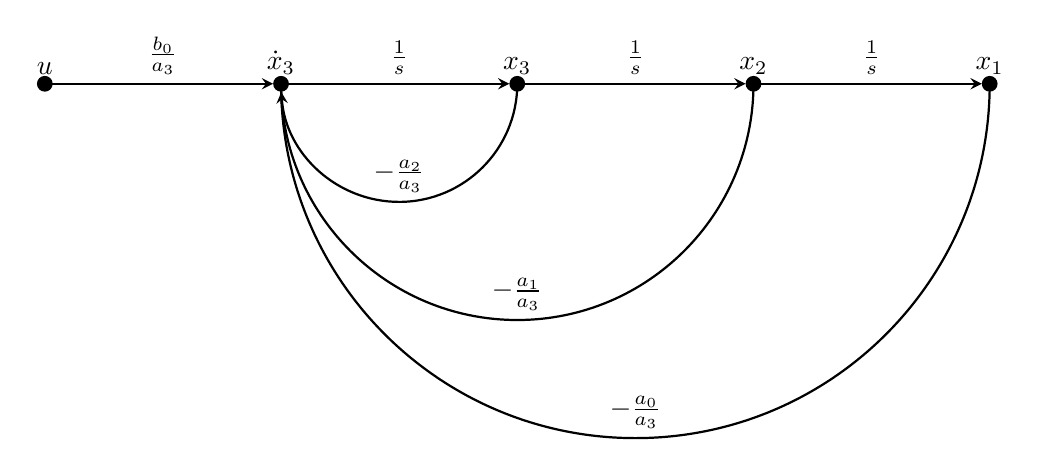
\begin{tikzpicture}[
      signal/.style={thick, ->},
      >=stealth
    ]
    \fill (0,0) circle (0.1) node[above] {$u$};
    \fill (3,0) circle (0.1) node[above] {$\dot{x}_3$};
    \fill (6,0) circle (0.1) node[above] {$x_3$};
    \fill (9,0) circle (0.1) node[above] {$x_2$};
    \fill (12,0) circle (0.1) node[above] {$x_1$};
    \draw[signal] (0,0) -- (2.9,0);
    \draw[signal] (3,0) -- (5.9,0);
    \draw[signal] (6,0) -- (8.9,0);
    \draw[signal] (9,0) -- (11.9,0);
    \node[above] at (1.5, 0) {$ \frac{b_0}{a_3} $};
    \node[above] at (4.5, 0) {$ \frac{1}{s} $};
    \node[above] at (7.5, 0) {$ \frac{1}{s} $};
    \node[above] at (10.5, 0) {$ \frac{1}{s} $};
    \draw[signal] (6, 0) arc (0:-176:1.5);
    \draw[thick] (9, 0) arc (0:-180:3);
    \draw[thick] (12, 0) arc (0:-180:4.5);
    \node[above] at (4.5, -1.5) {$ -\frac{a_2}{a_3} $};
    \node[above] at (6, -3) {$ -\frac{a_1}{a_3} $};
    \node[above] at (7.5, -4.5) {$ -\frac{a_0}{a_3} $};
  \end{tikzpicture}
\end{figure}
\end{document}
